\chapter{Lecture 4 - Homogeneous Linear Equations with Constant Coefficients}
\label{ch:lec4}
\section{Objectives}
The objectives of this lecture are:
\begin{itemize}
\item Review the solution methodology for homogeneous linear equations with constant coefficients.
\item Illustrate this method with several examples.
\end{itemize}
\section{Introduction}
In this lecture we will review the well-trod ground of your differential equations class and remind ourselves how to solve linear, constant coefficient, homogeneous, n\textsuperscript{th}-order differential equations.  These equations have the general form shown in Equation \ref{eq:lcchnode}:
\begin{equation}
a_nu^{(n)}+a_{n-1}u^{(n-1)}+\cdots+a_1u^{\prime}+a_0u=0
\label{eq:lcchnode}
\end{equation}
\noindent where the coefficients are real and constant an $a_n \ne 0$.

\newthought{The basic strategy} is to assume the solution is of the form: $u(x)=e^{mx}$. For the case of 2\textsuperscript{nd}-order equations, we get:\marginnote{If $u(x) = e^{mx}$ then, of course, $u^{\prime} = me^{mx}$ and $u^{\prime \prime} = m^2e^{mx}$.}
\begin{align*}
a_2m^2e^{mx}+a_1me^{mx}+a_0e^{mx}&=0 \\
e^{mx}\left(a_2m^2+a_1m+a_0\right)
\end{align*}
\noindent where the last line above is called the auxiliary equation: \marginnote{Here we re-name the constants so Equation \ref{eq:aux-eqn} takes a familiar form.}
\begin{equation}
am^2+bm+c = 0
\label{eq:aux-eqn}
\end{equation}
From the well-known quadratic equation, solutions are: $m = \frac{-b\pm\sqrt{b^2-4ac}}{2a}$
Solution of this equation gives the following three cases:
\begin{enumerate}
\item \textbf{Distinct Real Roots}
In this case $m_1 \ne m_2$ and the general solution is of the form:
\begin{equation}
u(x) = c_1\underbrace{e^{m_1x}}_{u_1(x)}+c_2\underbrace{e^{m_2x}}_{u_2(x)}
\label{eq:dist-real-roots}
\end{equation}

Using tools from the last lecture you should recognize that $u_1(x)$ and $u_2(x)$ are linearly independent for all $x\in \left( -\infty,\infty\right)$, and thus form a fundamental set of solutions.  

\newthought{An important special case} is when $m_1$ and $m_2$ are roots of a positive real number and thus $m_1 = -m_2$.  This happens when the governing equation is of the form:

\begin{equation}
u^{\prime \prime} - k^2 u = 0
\end{equation}
The general solution is:
\begin{equation}
u(x) = c_1 e^{-kx} + c_2e^{kx}
\label{eq:sp-case-1-exp}
\end{equation}
\begin{marginfigure}
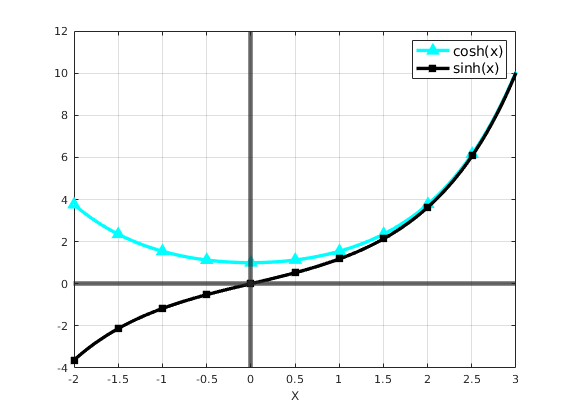
\includegraphics{cosh_and_sinh_plot.png}
\caption{Plot of $\cosh{x}$ and $\sinh{x}$}
\label{fig:cosh-and-sinh-plot}
\end{marginfigure}


For reasons that will become clear later in the course, it is sometimes useful to re-express the solution shown in Equation \ref{eq:sp-case-1-exp} in terms of the functions $\cosh{()}$ and $\sinh{()}$.  These functions are defined as linear combinations of exponentials as shown below and plotted in Figure \ref{fig:cosh-and-sinh-plot}.\marginnote{When applying boundary conditions and resolving unknown constants in a general solution to a differential equation, it is helpful that $\sinh{0} = 0$.  In contrast, neither $e^{x}$ nor $e^{-x}$ is equal to zero for finite values of $x$.}
\begin{align*}
\cosh{x} &= \frac{e^{x} + e^{-x}}{2} \\
\sinh{x} &= \frac{e^{x} - e^{-x}}{2}
\end{align*}



\item \textbf{Real Repeated Roots}
In this case $m_1 = m_2$.\marginnote{i.e. from the quadratic equation, $b^2-4ac = 0$}  One solution is:
\begin{equation}
u_1(x) = e^{m_1x}
\end{equation}

The other solution so derived is, of course, the same and thus we do not have two linearly independent solutions as required to form a fundamental set of solutions for a 2\textsuperscript{nd}-order linear homogeneous equation.  

\newthought{It can be shown} that a second linearly independent solution can be formed by multiplying $u_1(x)$ by the independent variable, $x$:\marginnote{This result is derived using a technique referred to as \emph{reduction of order}.  We will not take the time to cover it in this class (or in this book) but is concisely described in section 3.2 of Zill.  At a minimum you might at least confirm for yourself that a) $xu_1(x)$ is a solution to the equation; and b) use the Wronskian to confirm that it is linearly independent from $u_1(x)$.}
\begin{equation*}
u_2(x) = x u_1(x) = xe^{mx}
\end{equation*}
and thus the general solution for this case is:
\begin{equation}
u(x) = c_1e^{mx}+c_2xe^{mx}
\label{eq:rep-real-roots}
\end{equation}

\item \textbf{Conjugate Complex Roots}
In this case the discriminant, $b^2-4ac$, is negative so its square root is imaginary.  This results in $m_1$ and $m_2$ being complex conjugates which we will express as: $m_1 = \alpha + i\beta$ and $m_2 = \alpha - i\beta$.

The general solution is:
\begin{align*}
u(x) &= c_1e^{(\alpha + i\beta)x}+c_2e^{(\alpha - i\beta)x} \\
&=e^{\alpha x}\left(c_1e^{i\beta x} + c_2e^{-i\beta x} \right) 
\end{align*}

The complex exponentials in the last equation can be re-expressed using the Euler Formula:\index{Formula, Euler}
\begin{align*}
e^{i\beta x} &= \cos{\beta x} + i \sin{\beta x} \\
e^{-i\beta x} &= \cos{\beta x} - i \sin{\beta x}
\end{align*}
which is slightly more convenient insofar as the solutions are no longer expressed as complex exponentials; this expression also breaks the solutions down into their real and complex parts. It can be shown that both the real and imaginary parts of the solution must satisfy the differential equation \emph{independently}.  This fact allows us yet again to re-express the solution in a still more simple form that does not involve complex numbers at all:
\begin{equation}
u(x) = e^{\alpha x}\left(c_1 \cos{\beta x} + c_2 \sin{\beta x} \right)
\label{eq:cmplx-conj-roots}
\end{equation}

\newthought{Another important} special case is when the solution is \emph{pure imaginary} (i.e. $\alpha = 0$) so the solution is:
\begin{equation}
u(x) = c_1 \cos{\beta x} + c_2 \sin{\beta x}
\end{equation}
These solutions arise when the governing equation is as shown in Equation \ref{eq:special-case-2}:
\begin{equation}
u^{\prime \prime} + k^2 u = 0
\label{eq:special-case-2}
\end{equation}
The roots are $m_{1,2} = \pm ik$ and the general solution is:
\begin{equation}
u(x)=c_1 \cos{kx} + c_2 \sin{kx}
\end{equation}
This equation will be revisited throughout the course as it repeatedly comes up in applications.
\end{enumerate}

\section{Three Examples}
The cases described above will be illustrated with three examples:

\vspace{0.5cm}
\noindent\textbf{Example \#1:}
Find the general solution to $2u^{\prime \prime}-5u^{\prime}-3u = 0$. Inserting $u = e^{mx}$ into the equation gives us the auxiliary equation:
\begin{equation*}
2m^2 - 5m - 3 = (2m+1)(m-3)
\end{equation*}
with roots: $m_1 = -\frac{1}{2}$ and $m_2 = 3$.  These are real, distinct roots so the general solution is:
\begin{equation*}
u(x) = c_1e^{-x/2}+c_2e^{3x}
\end{equation*}

\vspace{0.5cm}

\noindent\textbf{Example \#2:}
Find the general solution to $u^{\prime \prime}-10u^{\prime}+25u = 0$.
The auxiliary equation is:
\begin{equation*}
m^2-10m+25 = (m-5)(m-5)
\end{equation*}
with (repeated) roots: $m_1 = 5$ and $m_2 = 5$.  These are real, repeated roots so the general solution is:
\begin{equation*}
u(x) = c_1e^{5x} + c_2xe^{5x}
\end{equation*}

\vspace{0.5cm}

\noindent\textbf{Example \#3:}
Find the general solution to $4u^{\prime \prime}+4u^{\prime} + 17u = 0, \ \ u(0)=-1, \ u^{\prime}(0)=2$.

This is an initial value problem\marginnote{We can see that it must be an \emph{initial} value problem because the conditions are both given at the same location, $x_0=0$.} with continuous (and constant) coefficients and with $a_2(x)\ne 0$ for all values of $x$.  We know from Theorem \ref{thm:IVP-exist-and-unique} that a unique solution exists.  We will first find the general solution, then apply the initial conditions to resolve the unknown coefficients to reveal the solution.

The auxiliary equation is:
\begin{align*}
4m^2+4m+17 &= 0 \\
\text{using the quadratic equation, gives us:} \\
\frac{-4 \pm \sqrt{16 - 4(4)(17)}}{2(4)} &= -\frac{1}{2} \pm \frac{\sqrt{-256}}{8}\\
&= -\frac{1}{2} \pm \frac{-16}{8} \\
&= -\frac{1}{2} \pm 2i
\end{align*}
This gives us complex conjugate roots and the general solution is:
\begin{equation*}
u(x) = e^{-x/2}\left(c_1 \cos{2x} + c_2 \sin{2x} \right)
\end{equation*}
Applying the initial condition $u(0)=-1$ gives us:
\begin{align*}
u(0) &= e^{0}\left(c_1 \cos{0} + c_2 \sin{0} \right) \\
&= 1(c_1(1)+c_2(0)) \\
&= c_1 = -1
\end{align*}
To apply the second initial condition we need to use the chain-rule and product rule to differentiate the general solution.  This gives us:
\begin{multline*}
u^{\prime}(x) = -\frac{1}{2}e^{-x/2}c_1\cos{2x}-2e^{-x/2}c_1\sin{2x} + \\
-\frac{1}{2}e^{-x/2}c_2\sin{2x}+2e^{-x/2}c_2\cos{2x}
\end{multline*}
Evaluating $u^{\prime}(0)$ and substituting $c_1 = -1$ gives us:
\begin{align*}
u^{\prime}(0) &= -\frac{1}{2}(1)(-1)(1) + (1)(2)c_2(1) \\
&= \frac{1}{2}+2c_2 = 2 \\
  \Rightarrow 2c_2 &= \frac{3}{2} \\
 c_2 &= \frac{3}{4}
\end{align*}
Both constants are now known and the unique solution is:
\begin{equation*}
u(x) = e^{-x/2}\left(-\cos{2x}+\frac{3}{4}\sin{2x} \right)
\end{equation*}
